\chapter{Introduction}
\label{chap:intro}

\section{Motivation}
\label{sec:motivation}

In recent years the area of Computer vision, also known as Machine vision has attracted interest both in academia and in commerce. Most major universities are offering computer vision courses and research degrees and conferences and journals are accepting more computer vision related papers. Computer vision combines a variety of subjects such as Artificial intelligence, Machine Learning, Image, Video and general Signal Processing and other areas from computer science and engineering. Recently we have seen more commercial uses of computer vision technology, such as augmented reality applications in home computers, mobile devices, and in home entertainment. In its early stages, computer vision was mainly used for robotics in an attempt to make an artificially intelligent machine that can “see” not only passively but actually understand the content of the information it gathers. In subsequent years computer vision research had been extended for uses in medical image processing, photography and cinema. The emergence of computer graphics in films along with the appearance of the personal computer that allowed the users to manipulate computer graphics and digital images, opened the path for new digital image processing methods to be developed and the area of computer vision got more involved in this process, since computer vision for robotics could not actually be applied in the industry yet. 
\par
Segmentation has always been a difficult problem in computer vision and numerous approaches to solve this problem have been developed and can be found in the literature. In the industry, specifically in cinema, segmentation of portions of a film frame plays crucial role for the creation of synthetic scenes. In the early analog years, film producers had to manually cut and composite objects on film frames to create synthetic scenes and later on in the digital age, methods were pioneered to digitally segment and composite objects in scenes \cite{compositing}. Computer vision is still a developing area and since it is already applied for commercial purposes, any contribution to it is welcome.

\section{History}
\label{sec:history}

As mentioned before, in the early digital years, the film industry started to seek ways to create visual effects and wanted to combine captured film frames with synthetic objects, scenes generated with computer graphics, or combine pre-existing scenes with others. \textit{Lucasfilm}, creators of the Star Wars movies were ahead of their time in terms of visual effects and made important contributions to the film industry. Specifically in 1984 \cite{compositing} they introduced a method for compositing four channel images using a matte component, or better known as \textit{alpha matte}. During the same period, computer graphics research had reached a point that computer generated imagery could effectively be used in movies. In 1996 \textit{Microsoft Research} introduced a method for separating foreground from background objects efficiently using a monochrome background \cite{blue}, also known as \textit{chroma key}. In most of the cases blue or green colours are used for the background, due to the fact that they are the furthest from human skin colour and also take advantage of \textit{bayer grid} properties. They also introduced the \textit{triangulation} method where the same foreground was photographed with different natural backgrounds in order to create the alpha matte \cite{blue}. Another contribution took place in 1999 \cite{environment} where transparent and translucent objects refractive properties were taken into account for the distortion of the background during compositing. From there on digital matting and compositing have been the most important factor for visual effects in movies. The emergence of image and video editing software took advantage of the same techniques, and digital image matting and compositing started to make its appearance in other areas such as photography. Recent matting research focuses on solving the problem of matting on natural images, where background colours are unknown. 

\section{Terminology}
\label{sec:terminology}

Matting is the process where given an image \textit{C}, the goal is to separate the foreground \textit{F} from the background \textit{B} and create an alpha matte $\alpha$. The alpha matte is usually a single channel image where \textit{0} values are considered background, \textit{1}’s are considered foreground and intermediate values are considered to be the blending factor for the fuzzy regions/mixed pixels in the image. Compositing is the process of using the estimated alpha matte to composite the foreground and fuzzy parts of the image to a new background. In this case the alpha matte plays the role of the fourth channel of the foreground image called alpha channel. The whole idea is formulated using equation (\ref{eq:composite_e}). 

\begin{equation} \label{eq:composite_e}
C=\alpha F+(1-\alpha)B
\end{equation}

Assuming that an image consists of three channels, red \textit{R}, green \textit{G} and blue \textit{B} and an alpha channel $\alpha$, the problem is severely under constrained with three equations and seven unknowns (\ref{eq:composite_ce}) and no single solution can be found. 

\begin{equation} \label{eq:composite_ce}
C_r=\alpha F_r+(1-\alpha)B_r,\;\; C_b=\alpha F_b+(1-\alpha)B_b,\;\; C_g=\alpha F_g+(1-\alpha)B_g
\end{equation}

Such a problem could be solved only with some prior information and so, in most natural image matting methods the concept of a trimap (Figure 1b) is introduced that can be either user provided, or generated automatically. The trimap is a single channel image that consist of three regions, definite foreground, definite background and unknown region. The unknown region usually consists of the edges of the object to be segmented in the image and the fuzzy regions such as hair, fur, motion blur etc.

\begin{figure}[t!]
\centering
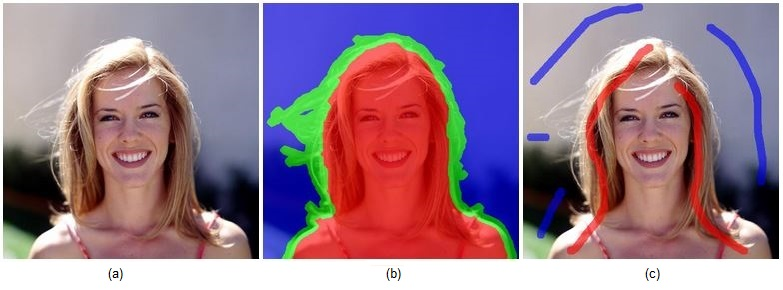
\includegraphics[width=0.9\columnwidth]{Chapter1/1/trimap.jpg}
\caption[Natural image, trimap and scribbles.]{A natural image, the trimap with definite foreground in red, definite background in blue and unknown region in green and an illustration of scribbles.}
\label{fig:trimap}
\end{figure}

\section{Overview of thesis}
\label{sec:overview-of-thesis}

The rest of the thesis is organized as follows: the following chapter is a literature review of various image matting methods, including fundamental methods such as blue screen matting, an in depth explanation of natural image matting methods starting from basic ones such as Bayesian matting and Closed Form matting and then a description of other important matting methods. The next section discusses state of the art matting methods, followed by a review of video matting techniques. The last section of the literature review consists of analysing matting methods with custom or specialized hardware. The next chapter gives a brief description of the development tools used for experimental implementation purposes. Chapter 4 describes all the preliminary work; the initial pre-existing algorithms used and early segmentation and matting algorithm formulations. A detailed description of the final algorithm and results from tests on benchmark images along with visual performance comparisons with other algorithms is done in Chapter 5. Chapter 6 presents an application of our algorithm using the Microsoft Kinect sensor, and a description of the extensions made to the algorithm for automatic trimap generation. Results are presented using images taken from the sensor, and visual performance comparisons are done with other algorithms. The final chapter consists of future work and conclusions.